\documentclass[12pt]{article}

\title{Activity 6: Encryption}
\author{Dr. Chris Mayfield}
\date{CS 101, Fall 2016}

%\ProvidesPackage{cspogil}

% fonts
\usepackage[utf8]{inputenc}
\usepackage[T1]{fontenc}
\usepackage{mathpazo}

% spacing
\usepackage[margin=2cm]{geometry}
\renewcommand{\arraystretch}{1.4}
\setlength{\parindent}{0pt}

% orphans and widows
\clubpenalty=10000
\widowpenalty=10000
\pagestyle{empty}

% figures and tables
\usepackage{graphicx}
\usepackage{multicol}
\usepackage{tabularx}
\usepackage{wrapfig}

% fixed-width columns
\usepackage{array}
\newcolumntype{L}[1]{>{\raggedright\let\newline\\\arraybackslash\hspace{0pt}}m{#1}}
\newcolumntype{C}[1]{>{\centering\let\newline\\\arraybackslash\hspace{0pt}}m{#1}}
\newcolumntype{R}[1]{>{\raggedleft\let\newline\\\arraybackslash\hspace{0pt}}m{#1}}

% include paths
\makeatletter
\def\input@path{{Models/}{../../Models/}}
\graphicspath{{Models/}{../../Models/}}
\makeatother

% colors
\usepackage[svgnames,table]{xcolor}
\definecolor{bgcolor}{HTML}{FAFAFA}
\definecolor{comment}{HTML}{007C00}
\definecolor{keyword}{HTML}{0000FF}
\definecolor{strings}{HTML}{B20000}

% table headers
\newcommand{\tr}{\bf\cellcolor{Yellow!10}}

% syntax highlighting
\usepackage{textcomp}
\usepackage{listings}
\lstset{
    basicstyle=\ttfamily\color{black},
    backgroundcolor=\color{bgcolor},
    numberstyle=\scriptsize\color{comment},
    commentstyle=\color{comment},
    keywordstyle=\color{keyword},
    stringstyle=\color{strings},
    columns=fullflexible,
    keepspaces=true,
    showlines=true,
    showstringspaces=false,
    upquote=true
}

% code environments
\newcommand{\java}[1]{\lstinline[language=java]{#1}}%[
\lstnewenvironment{javalst}{\lstset{language=java,backgroundcolor=}}{}
\lstnewenvironment{javabox}{\lstset{language=java,frame=single,numbers=left}\quote}{\endquote}

% PDF properties
\usepackage[pdftex]{hyperref}
\urlstyle{same}
\makeatletter
\hypersetup{
  pdftitle={\@title},
  pdfauthor={\@author},
  pdfsubject={\@date},
  pdfkeywords={},
  bookmarksopen=false,
  colorlinks=true,
  citecolor=black,
  filecolor=black,
  linkcolor=black,
  urlcolor=blue
}
\makeatother

% titles
\makeatletter
\renewcommand{\maketitle}{\begin{center}\LARGE\@title\end{center}}
\makeatother

% boxes [optional height]
\newcommand{\emptybox}[1][10em]{
\vspace{1em}
\begin{tabularx}{\linewidth}{|X|}
\hline\\[#1]\hline
\end{tabularx}}

% models
\newcommand{\model}[1]{\section{#1}\nopagebreak}
\renewcommand{\thesection}{Model~\arabic{section}}

% questions
\newcommand{\quest}[1]{\subsection*{Questions~ (#1)}}
\newcounter{question}
\newcommand{\Q}{\vspace{1em}\refstepcounter{question}\arabic{question}.~ }
\renewcommand{\thequestion}{\#\arabic{question}}

% sub-question lists
\usepackage{enumitem}
\setenumerate[1]{label=\alph*)}
\setlist{itemsep=1em,after=\vspace{1ex}}

% inline answers
\definecolor{answers}{HTML}{C0C0C0}
\newcommand{\ans}[1]{%
\ifdefined\Student
    \leavevmode\phantom{~~\textcolor{answers}{#1}}
\else
    ~~\textcolor{answers}{#1}
\fi}

% longer answers [optional height]
\newsavebox{\ansbox}
\newenvironment{answer}[1][4em]{
\nopagebreak
\begin{lrbox}{\ansbox}
\begin{minipage}[t][#1]{\linewidth}
\color{answers}
}{
\end{minipage}
\end{lrbox}
\ifdefined\Student
    \phantom{\usebox{\ansbox}}%
\else
    \usebox{\ansbox}%
\fi}


\begin{document}

\maketitle

\section*{Context: Security and Privacy}

We learned last week how easy it can be to examine network packets (e.g., using Wireshark) and how insecure the Internet can be.
As a team, brainstorm for a few minutes what activities people do online that they would like to be kept secure and/or private.
List several examples in the space below, and then have your presenter write the two most important on the whiteboard.

\emptybox

\model{Random Substitution}

Growing up, you likely decoded ``secret messages'' that simply used a different letter for each letter of the alphabet.
These types of encryption schemes can be broken easily using frequency analysis.
For example, we know that the letter E typically appears most frequently in English, followed by the letter T.
Consider the following famous quotation, encrypted using a random substitution:

\begin{center}
\bf PXL QLHP PXABCH AB OAGL KML GMLL
\end{center}


\quest{10 min}

\Q Count the frequency of each letter in the above quotation.

\begin{enumerate}
\setlength\itemsep{1em}

\item Which letter appears the most often? \ans{L (6 times)}

\item Which letter(s) appears the second most often? \ans{A and P (3 times)}

\item Which letter(s) appears the third most often? \ans{B, G, H, M, X (2 times)}

\end{enumerate}


\Q Now consider commonly used English words.

\begin{enumerate}
\setlength\itemsep{1em}

\item What are some commonly used three-letter words? \ans{and, for, the}

\item What are some commonly used two-letter words? \ans{in, of, to}

\item Based on your answers to the above two questions, and using trial and error, decrypt the above quotation.

\begin{answer}[2em]
\begin{center}
THE BEST THINGS IN LIFE ARE FREE
\end{center}
\end{answer}

\item Discuss as a group the process you just used to decrypt the message, and describe it here.

\begin{answer}[5em]
We first guessed that L was E, since that's the most common letter. Then we thought PXL was THE, and filled in the other T's, H's, and E's. We then guessed that AB was IN. At that point we guessed the entire sentence, and all the letters matched up.
\end{answer}

\end{enumerate}


% Based on Model 3 in "Activity 13 Encryption" by Helen Hu

\model{Caesar Cipher}

Julius Caesar famously used a ``Cipher Wheel'' to encrypt his messages to Cicero.
This website provides an electronic version of the cipher wheel:

\begin{center}
\url{http://cryptoclub.math.uic.edu/shiftcipher/shiftcipher.htm}
\end{center}

The Cipher Wheel uses a shift of the alphabet to determine which letters should be substituted.
The outer ring is the original characters in \textbf{plaintext} (the first row of characters); the inner ring is the encrypted characters in \textbf{ciphertext} (the second row of characters).

\begin{center}
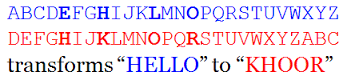
\includegraphics[height=0.65in]{CSP/caesar1.png}
\end{center}


\quest{15 min}


\Q In both the above model and in the electronic cypher wheel, blue (1st line) and red (2nd line) display the same set of characters.
Which color/line represents the original characters, and which color/line represents the encrypted characters?

\begin{answer}[3em]
Red is encrypted (ciphertext), and blue is original (plaintext).
\end{answer}


\Q Rotate the electronic cypher wheel to match the blue and red characters above, by clicking on the green arrows.
What is the key (the shift)?

\begin{answer}[3em]
The key is 3: A shifts to D, three letters to the right.
\end{answer}


\Q Assume we do not know the key, but we know a Caesar encryption was used to encrypt this following ciphertext.
Using trial and error, decrypt the phrase:

\begin{center}
PDA XAOP PDEJCO EJ HEBA WNA BNAA
\end{center}

\begin{enumerate}

\item What is the original text?
\ans{THE BEST THINGS IN LIFE ARE FREE}

\item What is the key (the shift)?
\ans{The key is 22: A shifts to W, three letters to the left.}

\end{enumerate}


\Q Consider how we might decrypt the phrase without the key.

\begin{enumerate}

\item How many different keys are there?

\ans{There are 26 keys; however, the key of zero is worthless.}

\item Describe the process that YOU used to decrypt a phrase when the key was unknown.

\begin{answer}
We guessed the first word might be THE, and then we lined up the wheel on cryptoclub to decrypt the rest.
\end{answer}

\item In contrast, describe the process a COMPUTER could use to decrypt a phrase when the key is unknown.

\begin{answer}
Computers can simply try all 26 keys, one by one.
They can also use a spell checker to see if the answer contains English words.
\end{answer}

\end{enumerate}


\Q Think about the examples you brainstormed at the beginning of the activity.
What is one advantage and one disadvantage of using Caesar Cipher encryption for online security?

\begin{enumerate}

\item one advantage: \ans{It's very simple and fast to compute.}

\item one disadvantage: \ans{It's very easy to guess the key.}

\end{enumerate}


\newpage

% Based on Model 4 in "Activity 13 Encryption" by Helen Hu

\model{Vigenère Cipher}

Vigenère Ciphers are a value-added Caesar Cipher that is very difficult to crack.
Instead of using a single number, the key is a word.
Each character in the key is encoded with its own Caesar Cipher.
For example, here is how you encrypt the word \texttt{UMBRELLA} using the key \texttt{DOG} shown below.

\begin{table}[h!]
\centering
\begin{tabular}{lll}
1. & Enter plaintext: & \texttt{UMBRELLA} \\[1ex]
2. & Apply the key:   & \texttt{DOGDOGDO} \\[1ex]
3. & Get ciphertext:  & \texttt{XAHUSROO}
\end{tabular}
\end{table}
\vspace{-1em}
\begin{center}
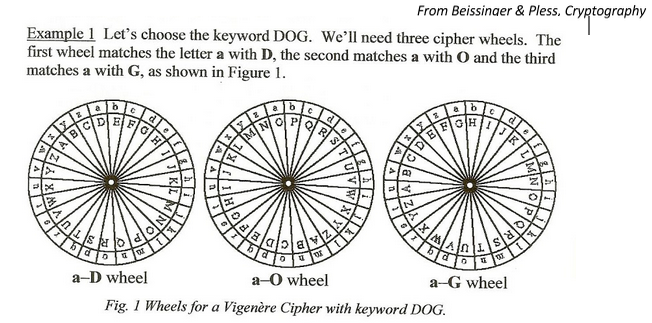
\includegraphics[width=0.9\linewidth]{CSP/vigenere1.png}
\end{center}

\quest{15 min}


\Q Which letters in \texttt{UMBRELLA} use:

\begin{enumerate}

\item the a-D wheel for encryption? \ans{U, R, L}

\item the a-O wheel for encryption? \ans{M, E, A}

\item the a-G wheel for encryption? \ans{B, L}

\end{enumerate}


\Q Why do you think the online cipher wheel uses lower-case letters for the outer wheel and upper-case letters for the inner wheel?

\begin{answer}
To make it easier to see the difference between plaintext and ciphertext.
\end{answer}


\Q If you were encrypting the word \texttt{PEANUT} using the keyword \texttt{CAT}, list which letters would use which cipher wheel.

\begin{answer}
\centering
C: P, N
\hspace{3em}
A: E, U
\hspace{3em}
T: A, T
\end{answer}


\Q Encrypt \texttt{PEANUT} using the keyword \texttt{CAT}.

\begin{answer}
\texttt{RETPUM} ~ (the first key is 2, the second is 0, the third is 19)
\end{answer}


\Q Consider the length of the keyword.

\begin{enumerate}

\item If we knew the keyword was two letters long, how many combinations of cipher wheels are there?
Show your work.

\ans{26 * 26 = 676}

\item If we knew the keyword was three letters long, how many combinations of cipher wheels are there?
Show your work.

\ans{26 * 26 * 26 = 17,576}

\item Ideally, if we needed to encrypt a 1000 character document, how long should the keyword be?
Explain your answer.

\begin{answer}
The longer the keyword, the more secure it is.
However, at some point it's not worth the extra computation.
Plus there's only 26 unique letters. 12-15 is practically enough.
\end{answer}

\end{enumerate}


\Q Think about the examples you brainstormed at the beginning of the activity.
What is one advantage and one disadvantage of using Vigenère Cipher encryption for online security?

\begin{enumerate}

\item one advantage:

\ans{It's still relatively simple to compute, and more secure than Caesar ciphers.}

\item one disadvantage:

\ans{The key is more complex, and it may be slower to perform the encryption.}

\end{enumerate}


\vfill

\section*{Conclusion}

Modern encryption techniques (e.g., RSA and AES) are much more sophisticated than the shift ciphers we've looked at in this activity.
But the idea is the same: you apply a ``key'' to some plaintext and transmit the resulting ciphertext.

\end{document}
